\section{Versuch 2 - Offsetbestimmung der Winkelgeschwindigkeiten}
Im zweiten Versuch wird die Würfelseite fixiert und die Winkelgeschwindigkeitswerte der beiden Sensoren aufgenommen. Hierbei werden jeweils $m = 1000$ Werte aufgenommen. Da der Sollwert $\dot{\varphi} = 0 \frac{m}{s}$ bekannt ist kann die systematische Messabweichung der Sensoren über den Mittelwert bestimmt werden. Der proportionale Umrechnungsfaktor von Rohdaten zu Winkelgeschwindigkeiten wird dem Datenblatt des Herstellers entnommen.

\begin{figure}[h]
	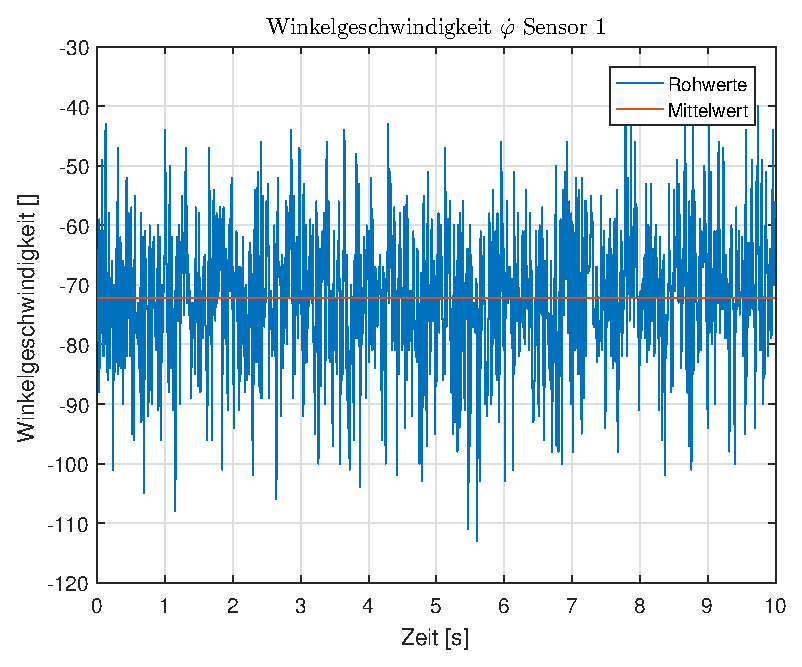
\includegraphics[width=0.5\linewidth]{img/phi1__d.eps}
	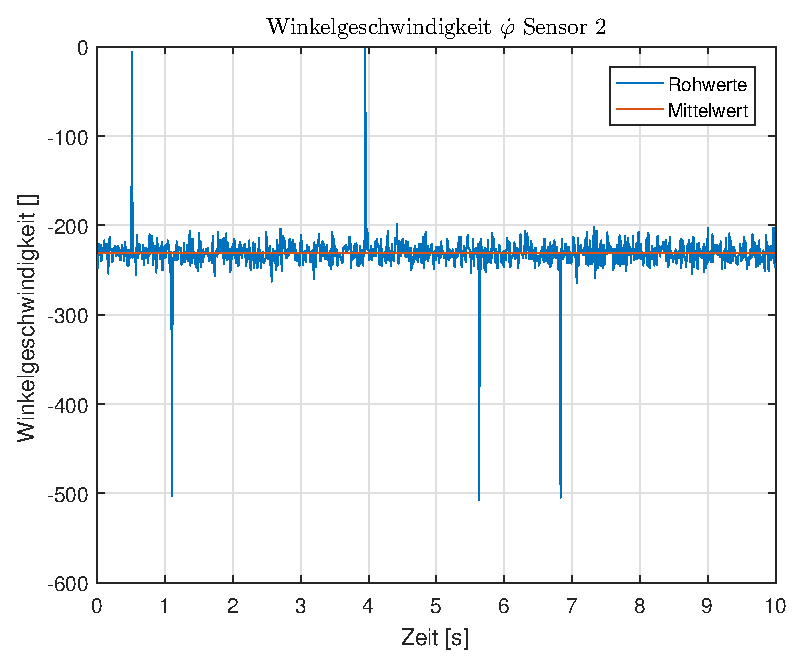
\includegraphics[width=0.5\linewidth]{img/phi2__d.eps}
\end{figure}

\begin{equation}
\dot{\varphi}_n = p^1_{\dot{\varphi}_n}  \cdot (\dot{\varphi}_n + p^2_{\dot{\varphi}_n})
\end{equation}

\begin{table}[h]
\centering
\begin{tabular}{lcllcl}
$p^1_{\varphi_1}$ &$=$& $-0.0076$ & $p^2_{\varphi_1}$ &$=$& $-72$ \\
$p^1_{\varphi_2}$ &$=$& $-0.0076$ & $p^2_{\varphi_2}$ &$=$& $-231$ \\
\end{tabular}
\end{table}